\documentclass[sigplan,10pt,authorversion]{acmart}

\usepackage[T1]{fontenc}
\usepackage[utf8]{inputenc}

\usepackage{acronym} % \ac[p], \acl[p], \acs[p], \acf[p]
\usepackage{algorithm} % \begin{algorithm} \end{algorithm}
\usepackage{algpseudocode} % \begin{algorithmic} \end{algorithmic}
\algnewcommand{\LeftComment}[1]{$\triangleright$ #1}

\usepackage[inline]{enumitem} % \begin{enumerate*} \end{enumerate*}
\usepackage{tikz} % \begin{tikzpicture} \end{tikzpicture}

\usepackage{graphicx}
\usepackage{color}
\AtBeginDocument{
\definecolor{pdfurlcolor}{rgb}{0,0,0}
\definecolor{pdfcitecolor}{rgb}{0,0,0}
\definecolor{pdflinkcolor}{rgb}{0,0,0}
\definecolor{light}{gray}{.85}
\definecolor{vlight}{gray}{.95}
\definecolor{darkgreen}{rgb}{0.0, 0.2, 0.13}
\definecolor{mydarkblue}{RGB}{116,173,209}
\definecolor{mydarkblueid}{RGB}{83,154,198}
\definecolor{mylightblue}{RGB}{171,217,233}
\definecolor{mydarkorange}{RGB}{244,109,67}
\definecolor{mylightorange}{RGB}{252,153,54}
\definecolor{mydarkred}{RGB}{215,48,39}
}


\usepackage[draft,inline,nomargin,index]{fixme}
\fxsetup{theme=colorsig,mode=multiuser,inlineface=\itshape,envface=\itshape}
\FXRegisterAuthor{go}{ago}{Gerald}
\FXRegisterAuthor{mn}{amn}{Matthieu}

\usepackage{subcaption} % subfigure

% Commands
%---------
\newcommand{\ie}{i.e. }

\newcommand{\inbb}[1]{\in \mathbb{#1}}
\newcommand{\mathlist}[2]{\set{#1_i \in #2}_{i \inbb{N}}}
\newcommand{\trm}[1]{\mathit{#1}}
\newcommand{\set}[1]{\left\{#1\right\}} % set brace notation

\newcommand{\id}[3]{$\trm{#1}^{\trm{#2}}_{\trm{#3}}$}

\newcommand{\widthletter}{7mm}
\newcommand{\widthblock}{11mm}

% Tikz styles
\tikzset{
    common/.style={anchor=west, draw, rectangle, minimum height=6mm},
    letter/.style={common, minimum width=\widthletter},
    block/.style={common, minimum width=\widthblock},
    cross/.style={
        path picture={
            \draw[mydarkred, very thick]
                (path picture bounding box.south east)--(path picture bounding box.north west)
                (path picture bounding box.south west)--(path picture bounding box.north east);
        }
    }
}

% Acronyms
% --------
\acrodef{ADT}[ADT]{Abstract Data Type}
\acrodefplural{ADT}[ADTs]{Abstract Data Types}
\acrodef{CRDT}[CRDT]{Conflict-free Replicated Data Type}
\acrodefplural{CRDT}[CRDTs]{Conflict-free Replicated Data Types}
\acrodef{JIT}[JIT]{Just-In-Time}
\acrodef{OT}[OT]{Operational Transformation}
\acrodefplural{OT}[OT]{Operational Transformations}
\acrodef{P2P}[P2P]{Peer-to-Peer}
\acrodef{SEC}[SEC]{Strong Eventual Consistency}

% Additional config
% --------
\bibliographystyle{unsrtnat}
\def\algorithmautorefname{Algorithm} % \autoref
\hyphenation{Renamable-LogootSplit}

\begin{document}

\title{Efficient Renaming in Sequence CRDTs}

\author{Matthieu Nicolas}
\email{matthieu.nicolas@loria.fr}
\affiliation{%
  \institution{Université de Lorraine, CNRS, Inria, LORIA, F-54500}
  \city{Nancy}
  \country{France}
}

\author{Gérald Oster}
\email{gerald.oster@loria.fr}
\affiliation{%
  \institution{Université de Lorraine, CNRS, Inria, LORIA, F-54500}
  \city{Nancy}
  \country{France}
}

\author{Olivier Perrin}
\email{olivier.perrin@loria.fr}
\affiliation{%
  \institution{Université de Lorraine, CNRS, Inria, LORIA, F-54500}
  \city{Nancy}
  \country{France}
}

% Pre-print settings
\settopmatter{printacmref=false}
\renewcommand\footnotetextcopyrightpermission[1]{} % removes footnote with conference information in first column
\pagestyle{plain} % removes running headers

% PaPoc'20 settings
% \acmConference[PaPoC '20]{7th Workshop on Principles and Practice of Consistency for Distributed Data}{April 27, 2020}{Heraklion, Crete, Greece}

\begin{abstract}
To achieve high availability, large-scale distributed systems have to replicate data and to minimise coordination between nodes.
Literature and industry increasingly adopt \acfp{CRDT} to design such systems.
\acp{CRDT} are data types which behave as traditional ones, e.g. the Set or the Sequence.
However, unlike traditional data types, they are designed to natively support concurrent modifications.
To this end, they embed in their specification a conflict-resolution mechanism.

To resolve conflicts in a deterministic manner, \acp{CRDT} usually attach identifiers to elements stored in the data structure.
Identifiers have to comply with several constraints, such as uniqueness or belonging to a dense order.
These constraints may hinder the identifiers’ size from being bounded.
As the system progresses, identifiers tend to grow.
This inflation deepens the overhead of the \ac{CRDT} over time, leading to performance issues.

To address this issue, we propose a new CRDT for Sequence which embeds a renaming mechanism.
It enables nodes to reassign shorter identifiers to elements in an uncoordinated manner.
Experimental results demonstrate that this mechanism decreases the overhead of the replicated data structure and eventually limits it.
\end{abstract}

\begin{CCSXML}
    <ccs2012>
        <concept>
            <concept_id>10003752.10003809.10010172</concept_id>
            <concept_desc>Theory of computation~Distributed algorithms</concept_desc>
            <concept_significance>500</concept_significance>
        </concept>
        <concept>
            <concept_id>10010405.10010497.10010500.10010501</concept_id>
            <concept_desc>Applied computing~Text editing</concept_desc>
            <concept_significance>500</concept_significance>
        </concept>
        <concept>
            <concept_id>10003120.10003130.10003233</concept_id>
            <concept_desc>Human-centered computing~Collaborative and social computing systems and tools</concept_desc>
            <concept_significance>100</concept_significance>
        </concept>
        <concept>
            <concept_id>10011007.10010940.10010992.10010993.10010996</concept_id>
            <concept_desc>Software and its engineering~Consistency</concept_desc>
            <concept_significance>100</concept_significance>
        </concept>
    </ccs2012>
\end{CCSXML}
\ccsdesc[500]{Theory of computation~Distributed algorithms}
\ccsdesc[500]{Software and its engineering~Consistency}
\ccsdesc[100]{Human-centered computing~Collaborative and social computing systems and tools}
\ccsdesc[100]{Applied computing~Text editing}

\keywords{CRDTs, real-time collaborative editing, eventual consistency, memory-wise optimisation, performance}

\maketitle

\section{Introduction}

In order to serve an ever-growing number of users and provide an increasing volume of data, large-scale systems such as data stores or collaborative editing tools adopt the \emph{eventual consistency} model \cite{10.1145/224057.224070}.
This model ensures the high availability of the system, even in case of network partitions.
To this end, it relaxes consistency constraints and minimises coordination between nodes.
In this model, every node owns a copy of the data, can modify it and propagate the updates to others.
Therefore, replicas can temporarily diverge.
To ensure that nodes converge eventually despite concurrently generated updates, a conflict resolution mechanism is required.

Several approaches were introduced to design efficient conflict resolution mechanisms.
The one we consider proposes to use \acfp{CRDT} \cite{shapiro_2011_crdt}.
\acp{CRDT} are new specifications of abstract data types, e.g. the Set or the Sequence.
However, when compared to former ones, they are designed to support natively concurrent modifications.
To this end, they embed a conflict-resolution mechanism directly in their specification.

\acp{CRDT} appear as a keystone technology of a new paradigm of applications: Local-First Software \cite{10.1145/3359591.3359737}.
They also have been proven a suitable approach to build distributed real-time collaborative editors \cite{doi:10.1002/cpe.4108}.
Still, they exhibits some limitations.
Especially in the context of real-time collaborative editing, the internal conflict resolution mechanism accumulates a large amount of metadata over time.

To address this particular issue, we propose a new \ac{CRDT} for Sequence which embeds a renaming mechanism.
It enables to minimise the overhead of the data structure by discarding accumulated metadata eventually.

This paper is organised as follows.
Section \ref{sec:background} provides the background of our approach.
In \autoref{sec:proposition}, we introduce \emph{RenamableLogootSplit}, our new \ac{CRDT} for Sequence.
Section \ref{sec:evaluation} presents the benchmarks we performed to evaluate our proposition and the obtained results.
In \autoref{sec:related-work}, we compare our approach to existing ones.
Finally, \autoref{sec:conclusion} concludes and introduces possible future work.

\section{Background}
\label{sec:background}

To deterministically solve conflicts and ensure convergence of all nodes, \acp{CRDT} rely on metadata.
In the context of Sequence \acp{CRDT}, two different approaches were proposed, both trying to minimise the overhead introduced.
The first one \cite{oster:inria-00108523, ROH2011354,briot:hal-01343941} attaches fixed size identifiers to each element in the sequence and uses them to represent the sequence as a linked list.
The downside of this approach is an ever growing overhead, as it needs to keep removed elements to deal with potential concurrent updates, effectively turning them into tombstones.
The second one \cite{5158449,WeissICDCS09,AndreCollaborateCom2013} avoids the need of tombstones by attaching identifiers from a dense totally ordered set to elements.
Elements are ordered into the sequence by comparing their respective identifiers.
However this approach suffers from an ever-increasing overhead, as the size of such dense totally ordered identifiers is variable and grows over time.
In the context of this paper, we focus on the later approach.

\subsection{LogootSplit}

Proposed by \citet{AndreCollaborateCom2013}, LogootSplit (LS) is the state of the art of the variable-size identifiers approach of Sequence \ac{CRDT}.
As explained previously, it uses identifiers from a dense totally ordered set to position elements into the replicated sequence.

To this end, LogootSplit generates identifiers made of a list of tuples to elements.
These tuples have four components:
\begin{enumerate*}
    \item a \emph{position}, which embodies the intended position of the element
    \item a \emph{node identifier},
    \item a \emph{node sequence number} and
    \item an \emph{offset}, which are combined to make identifiers unique.
\end{enumerate*}
By comparing identifiers using the lexicographical order, LogootSplit is able to determine the position of the element relatively to others.
In this paper, we represent identifiers using the following notation: \id{position}{node~id~node~seq}{offset} where $\trm{position}$ is a lowercase letter, $\trm{node~id}$ an uppercase one and both $\trm{node~seq}$ and $\trm{offset}$ integers.

Instead of storing an identifier for each element of the sequence, the main insight of LogootSplit is to aggregate dynamically elements into blocks.
Grouping elements into blocks enables LogootSplit to assign logically an identifier to each element while effectively storing only the block length and the identifier of its first element.
LogootSplit gathers elements with \emph{contiguous} identifiers into a block.
We call \emph{contiguous} two identifiers that are identical except for their last offset, and with both offsets being consecutive.
\autoref{fig:logootsplit-seq} illustrates such a case: in \autoref{fig:logootsplit-seq-as-letters}, the element identifiers form a chain of contiguous identifiers.
LogootSplit is then able to group them into one block to minimise the metadata stored, as shown in \autoref{fig:logootsplit-seq-as-block}.

\begin{figure}[ht!]
    \begin{subfigure}{0.38\columnwidth}
        \centering
        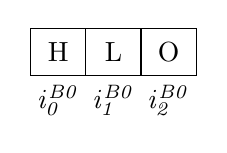
\begin{tikzpicture}
            \path
                node[letter, label=below:{\id{i}{B0}{0}}] {H}
                to ++(0:\widthletter) node[letter, label=below:{\id{i}{B0}{1}}] {L}
                to ++(0:\widthletter) node[letter, label=below:{\id{i}{B0}{2}}] {O};
        \end{tikzpicture}
        \caption{Elements with their corresponding identifiers}
        \label{fig:logootsplit-seq-as-letters}
    \end{subfigure}
    \hspace{0.03\columnwidth}
    \begin{subfigure}{0.45\columnwidth}
        \centering
        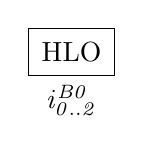
\begin{tikzpicture}
            \path
                node[block, label=below:{\id{i}{B0}{0..2}}] {HLO};
        \end{tikzpicture}
        \caption{Elements grouped into a block}
        \label{fig:logootsplit-seq-as-block}
    \end{subfigure}
    \caption{Representation of a LogootSplit sequence containing the elements "HLO"}
    \label{fig:logootsplit-seq}
\end{figure}

This feature allows to shift the root of metadata growth from the number of elements to the number of blocks.
As blocks can contain an arbitrary number of elements, it enables to reduce significantly the memory overhead of the data structure.

\subsection{Limits}

As stated previously, the size of identifiers from a dense totally ordered set is variable.
When nodes insert new elements between two others with the same \emph{position} value, LogootSplit has no other option than to increase the size of the resulting identifiers.
\autoref{fig:example-split} illustrates such cases.
In this example, since the node inserts a new element between contiguous identifiers, LogootSplit is not able to generate a fitting identifier of the same size.
To comply with the intended order, LogootSplit generates a new identifier by appending a new tuple to the identifier of the predecessor.

\begin{figure}[ht!]
    \centering
    \begin{tikzpicture}
        \path
            node {\textbf{A}}
            to ++(0:\widthletter) node[block, label=below:{\id{i}{B0}{0..2}}] (HLO) {HLO}
            to ++(0:5 * \widthletter) node[letter, label=below:{\id{i}{B0}{0}}] (H) {H}
            to ++(0:\widthletter) node[letter, fill=mydarkorange, label=above:{\color{mydarkorange}\id{i}{B0}{0}\id{f}{A0}{0}}] {E}
            to ++(0:\widthletter) node[block, label=below:{\id{i}{B0}{1..2}}] {LO};

        \draw[->, thick] (HLO) -- node[below, align=center]{\emph{insert "e"}\\\emph{between}\\\emph{"h" and "l"}} (H);
    \end{tikzpicture}
    \caption{Insertion leading to longer identifiers}
    \label{fig:example-split}
\end{figure}

As a result, the size of identifiers tends to grow as the collaboration progresses.
This growth impacts negatively performance of the data structure on several aspects.
Since identifiers attached to values become longer, the memory overhead of the data structure increases accordingly.
This also increases the bandwidth consumption as nodes have to broadcast identifiers to others.

Additionally, as the lifetime of the replicated sequence increases, the number of blocks composing it grows as well.
Indeed, several constraints on identifier generation prevent nodes from adding new elements to existing blocks.
For example, only the node that generated the block can append or prepend elements to it.
These limitations cause the generation of new blocks.
Since no mechanism to merge blocks a posteriori is provided, the sequence ends up fragmented into many blocks.
The efficiency of the data structure decreases as each block introduces its own overhead.

In our benchmarks, we measure that the content eventually represents less than 1\% of the data structure size, the remaining 99\% being metadata.
It is thus necessary to address the previously highlighted issues.

\section{Proposed approach}
\label{sec:proposition}

We propose a new Sequence \ac{CRDT} belonging to the variable-size identifiers approach: \emph{RenamableLogootSplit} (RLS) \cite{nicolas:hal-01932552}.

To address the limitations of LogootSplit, we embed in the data structure a renaming mechanism.
The purpose of this mechanism is to reassign shorter identifiers to elements and to group them into blocks to minimise the memory overhead of the whole sequence.

To avoid costly and blocking consensus algorithms, we instead adopt the \emph{optimistic replication} \cite{10.1145/1057977.1057980} approach for our mechanism.
Nodes perform renaming without any coordination.
However, this operation is not intrinsically commutative with others.
If conflicts arise, we use \emph{Operational Transformations} (OT) \cite{10.1145/289444.289469,4668339} to enable nodes to resolve them deterministically.

\subsection{System Model}

The system is composed of a dynamic set of nodes, as nodes join and leave dynamically the collaboration during its lifetime.
Nodes collaborate to build and maintain a sequence using RenamableLogootSplit.
Each node owns a copy of the sequence and edit it without any coordination.

Nodes communicate through a \ac{P2P} network, which is unreliable.
Messages can be lost, re-ordered or delivered multiple times.
The network is also vulnerable to partitions, which split nodes into disjoined subgroups.
To overcome the failures of the network, nodes rely on a message-passing layer.
As RenamableLogootSplit is built on top of LogootSplit, it shares the same requirements for the operation delivery.
This layer is thus used to deliver messages to the application exactly-once.
The layer also ensures that \emph{remove} operations are delivered after corresponding \emph{insert} operations.
Nodes use an anti-entropy mechanism to synchronise in a pairwise manner, by detecting and re-exchanging lost operations.

\subsection{\emph{rename} operation}

\label{sec:rename-op}

Our \emph{rename} operation helps RenamableLogootSplit to reduce the overhead of nodes replica.
This operation reassigns arbitrary identifiers to elements.

\begin{figure}[ht!]
    \begin{subfigure}{\columnwidth}
        \begin{tikzpicture}
            \path
                node {\textbf{A}}
                to ++(0:\widthletter) node[letter, label=below:{\id{i}{B0}{0}}] {H}
                to ++(0:\widthletter) node[letter, fill=mydarkorange, label=above:{\color{mydarkorange}\id{i}{B0}{0}\id{f}{A0}{0}}] {E}
                to ++(0:\widthletter) node[block, label=below:{\id{i}{B0}{1..2}}] (LO) {LO}
                to ++(0:4 * \widthletter) node[letter, fill=mydarkblue, label=below:{\color{mydarkblueid}\id{i}{A1}{0}}] (H) {H};

            \draw[->, thick] (LO) -- node[below, align=center]{\emph{rename}} (H);
        \end{tikzpicture}
        \caption{Selecting the new identifier of the first element}
        \label{fig:renaming-first-id}
    \end{subfigure}
    \begin{subfigure}{\columnwidth}
        \begin{tikzpicture}
            \path
                node {\textbf{A}}
                to ++(0:\widthletter) node[letter, label=below:{\id{i}{B0}{0}}] {H}
                to ++(0:\widthletter) node[letter, fill=mydarkorange, label=above:{\color{mydarkorange}\id{i}{B0}{0}\id{f}{A0}{0}}] {E}
                to ++(0:\widthletter) node[block, label=below:{\id{i}{B0}{1..2}}] (LO) {LO}
                to ++(0:4 * \widthletter) node[letter, fill=mydarkblue, label=below:{\color{mydarkblueid}\id{i}{A1}{0}}] (H) {H}
                to ++(0:\widthletter) node[letter, fill=mydarkblue, label=below:{\color{mydarkblueid}\id{i}{A1}{1}}] {E}
                to ++(0:\widthletter) node[letter, fill=mydarkblue, label=below:{\color{mydarkblueid}\id{i}{A1}{2}}] {L}
                to ++(0:\widthletter) node[letter, fill=mydarkblue, label=below:{\color{mydarkblueid}\id{i}{A1}{3}}] {0};

                \draw[->, thick] (LO) -- node[below, align=center]{\emph{rename}} (H);
            \end{tikzpicture}
            \caption{Selecting the new identifiers of the remaining ones}
        \label{fig:renaming-second-id}
    \end{subfigure}
    \begin{subfigure}{\columnwidth}
        \begin{tikzpicture}
            \path
                node {\textbf{A}}
                to ++(0:\widthletter) node[letter, label=below:{\id{i}{B0}{0}}] {H}
                to ++(0:\widthletter) node[letter, fill=mydarkorange, label=above:{\color{mydarkorange}\id{i}{B0}{0}\id{f}{A0}{0}}] {E}
                to ++(0:\widthletter) node[block, label=below:{\id{i}{B0}{1..2}}] (LO) {LO}
                to ++(0:4 * \widthletter) node[block, fill=mydarkblue, label=below:{\color{mydarkblueid}\id{i}{A1}{0..3}}] (HELO) {HELO};

            \draw[->, thick] (LO) -- node[below, align=center]{\emph{rename}} (HELO);
        \end{tikzpicture}
        \caption{Final state obtained}
        \label{fig:renaming-final-state}
    \end{subfigure}
    \caption{Renaming the sequence on node \emph{A}}
    \label{fig:renaming}
\end{figure}

Its behaviour is illustrated in \autoref{fig:renaming}.
In this example, node A initiates a \emph{rename} operation on its local state.
First, node A reuses the id of the first element of the sequence (\id{i}{B0}{0}) but modifies it with its own node id (\textbf{A}) and current sequence number (\emph{1}).
Also the offset is set to 0.
Node A reassigns the resulting id (\id{i}{A1}{0}) to the first element of the sequence as described in \autoref{fig:renaming-first-id}.
Then, node A derives contiguous identifiers for all remaining elements by successively incrementing the offset (\id{i}{A1}{1}, \id{i}{A1}{2} and \id{i}{A1}{3}), as shown in \autoref{fig:renaming-second-id}.
As we assign contiguous identifiers to all elements of the sequence, we eventually group them into one block as illustrated in \autoref{fig:renaming-final-state}.
It allows nodes to benefit the most from the block feature and to minimise the overhead of the resulting state.

To eventually converge, other nodes have to rename their state identically.
However, they can not simply replace their current state with the new renamed one.
Indeed, they may have performed concurrent updates on their states.
To not discard these updates, nodes have to process the \emph{rename} operation themselves.
To this end, the node issuing the \emph{rename} operation broadcasts its former state to others.
Using the former state, other nodes compute the new identifier of each renamed identifier.
As for concurrently inserted identifiers, we will explain in \autoref{sec:dealing-with-concurrent-updates} how nodes rename them in a deterministic way.

To limit bandwidth consumption of \emph{rename} operations, we propose a compression technique to broadcast only necessary components to uniquely identify blocks instead of whole identifiers.
It reduces the data to send to a fixed amount per block.
Additionally, we can set an upper-bound to the size of \emph{rename} operations by issuing them as soon as the state reaches a given number of blocks.

\subsection{Dealing with concurrent updates}

\label{sec:dealing-with-concurrent-updates}

As \emph{rename} operations can be issued without any kind of coordination, it is possible for other nodes to perform updates concurrently.
Figure \ref{fig:concurrent-insert-rename-inconsistent} illustrates such cases.
In this example node B inserts the new element "L", assigns the id \id{i}{B0}{0}\id{m}{B1}{0} to it and broadcasts its update, concurrently to the \emph{rename} operation described in \autoref{fig:renaming}.
Upon reception of the \emph{insert} operation, node A adds the inserted element into its sequence, using the element id to determine its position.
However, since identifiers were modified by the concurrent \emph{rename} operation, node A inserts the new element at the end of its sequence (since \id{i}{A1}{3} < \id{i}{B0}{0}\id{m}{B1}{0}) instead of at the intended position.
As described by this example, applying naively concurrent updates would result in inconsistencies.
It is thus necessary to handle concurrent operations to \emph{rename} operations in a particular manner.

\begin{figure}[ht!]
    \centering
    \begin{tikzpicture}
        \path
            node[label=below:{(after renaming)}] {\textbf{A}}
            to ++(0:2 * \widthletter) node[block, fill=mydarkblue, label=below:{\color{mydarkblueid}\id{i}{A1}{0..3}}] (HELO) {HELO}
            to ++(0:4 * \widthletter) node[block, fill=mydarkblue, label=below:{\color{mydarkblueid}\id{i}{A1}{0..3}}]  {HELO}
            to ++(0:\widthblock) node[cross, letter, fill=mylightorange, label=above:{\color{mylightorange}\id{i}{B0}{0}\id{m}{B1}{0}}] (right) {L};

        \path
            to ++(270:2) node[label=below:{(before renaming)}]  {\textbf{B}}
            to ++(0:2*\widthletter) node[letter, label=below:{\id{i}{B0}{0}}] {H}
            to ++(0:\widthletter) node[letter, fill=mydarkorange, label=above:{\color{mydarkorange}\id{i}{B0}{0}\id{f}{A0}{0}}] {E}
            to ++(0:\widthletter) node[letter, fill=mylightorange, label=below:{\color{mylightorange}\id{i}{B0}{0}\id{m}{B1}{0}}] (left) {L}
            to ++(0:\widthletter) node[block, label=below:{\id{i}{B0}{1..2}}] {LO};

        \draw[dashed, ->, thick] (left.north) .. controls +(90:2 * \widthletter) and +(270:2 * \widthletter) .. node[below right, align=center]{\emph{insert}} (right.south);
    \end{tikzpicture}
    \caption{Concurrent update leading to inconsistency}
    \label{fig:concurrent-insert-rename-inconsistent}
\end{figure}

To detect them, we use an \emph{epoch-based} system.
We add an \emph{epoch} to the sequence as a property.
Each time a \emph{rename} operation is applied, the sequence progresses to a new epoch.
When nodes issue operations, they tag them with their current epoch.
Upon the reception of an operation, nodes compare the operation epoch to their current one.
If they differ, nodes have to transform the operation before applying it.

\autoref{alg:renameId} enables nodes to transform \emph{insert} or \emph{remove} operations against the \emph{rename} one.
The main idea of this algorithm is to use the predecessor of the given identifier to do so.
An example of its usage is illustrated in \autoref{fig:concurrent-insert-rename-fixed}.
This figure depicts the same scenario as in \autoref{fig:concurrent-insert-rename-inconsistent}, except that this time node A uses \autoref{alg:renameId} to rename the concurrently generated id before inserting it in its state.
The algorithm proceeds as follows.
First, node A retrieves the predecessor of the given id \id{i}{B0}{0}\id{m}{B1}{0} in the former state: \id{i}{B0}{0}\id{f}{A0}{0}.
Then it computes the counterpart of \id{i}{B0}{0}\id{f}{A0}{0} in the renamed state: \id{i}{A1}{1}.
Finally, node A prepends it to the given id to generate the renamed id: \id{i}{A1}{1}\id{i}{B0}{0}\id{m}{B1}{0}.
By reassigning this id to the concurrently added element, node A is able to insert it in its state while preserving the intended order.

\begin{figure}[ht!]
    \centering
    \begin{tikzpicture}
        \path
            node[label=below:{(epoch 1)}] {\textbf{A}}
            to ++(0:2 * \widthletter) node[block, fill=mydarkblue, label=below:{\color{mydarkblueid}\id{i}{A1}{0..3}}] (HELO) {HELO}
            to ++(0:4 * \widthletter) node[block, fill=mydarkblue, label=below:{\color{mydarkblueid}\id{i}{A1}{0..1}}]  {HE}
            to ++(0:\widthblock) node[letter, fill=mylightblue, label=above:{\color{mylightblue!20!mydarkblueid}\id{i}{A1}{1}\id{i}{B0}{0}\id{m}{B1}{0}}] (right) {L}
            to ++(0:\widthletter) node[block, fill=mydarkblue, label=below:{\color{mydarkblueid}\id{i}{A1}{2..3}}]  {LO};


        \path
            to ++(270:2) node[label=below:{(epoch 0)}] {\textbf{B}}
            to ++(0:1.5 * \widthletter) node[letter, label=below:{\id{i}{B0}{0}}] {H}
            to ++(0:\widthletter) node[letter, fill=mydarkorange, label=above:{\color{mydarkorange}\id{i}{B0}{0}\id{f}{A0}{0}}] {E}
            to ++(0:\widthletter) node[letter, fill=mylightorange, label=below:{\color{mylightorange}\id{i}{B0}{0}\id{m}{B1}{0}}] (left) {L}
            to ++(0:\widthletter) node[block, label=below:{\id{i}{B0}{1..2}}] {LO};

        \draw[dashed, ->, thick] (left.north) .. controls +(90:2 * \widthletter) and +(270:2 * \widthletter) .. node[below right, align=center]{\emph{rename}\\ \emph{then insert}}(right.south);
    \end{tikzpicture}
    \caption{Renaming concurrent update using \autoref{alg:renameId} before applying it to maintain intended order}
    \label{fig:concurrent-insert-rename-fixed}
\end{figure}

\begin{algorithm}
    \caption{Rename concurrently generated identifier}
    \label{alg:renameId}
    \begin{algorithmic}
    \Function{renameId}{$\trm{id}, \trm{renamedBlocks}, \trm{nId}, \trm{nSeq}$}
        \Statex \LeftComment{$\trm{id}$ is the identifier to rename}
        \Statex \LeftComment{$\trm{renamedBlocks}$ is the former state}
        \Statex \LeftComment{$\trm{nId}$ is $\trm{node~id}$ of the node which issued the \emph{rename} op}
        \Statex \LeftComment{$\trm{nSeq}$ is $\trm{node~seq}$ of the node which issued the \emph{rename} op}\\

        \State $\trm{length} \gets \trm{renamedBlocks.length}$
        \State $\trm{firstId} \gets \trm{idBegin}(\trm{renamedBlocks}[0])$
        \State $\trm{lastId} \gets \trm{idEnd}(\trm{renamedBlocks}[\trm{length} - 1])$\\

        \State $\trm{pos} \gets \trm{position(firstId)}$
        \State $\trm{newFirstId} \gets \trm{new} \ \trm{Id}(\trm{pos}, \trm{nId}, \trm{nSeq}, 0)$
        \State $\trm{newLastId} \gets \trm{new} \ \trm{Id}(\trm{pos}, \trm{nId}, \trm{nSeq}, \trm{length - 1})$\\

        \If{$\trm{firstId} < \trm{id}$ \textbf{and} $\trm{id} < \trm{lastId}$}
            \State $\trm{pred} \gets \trm{findPredecessor}(\trm{id}, \trm{renamedBlocks})$
            \State $\trm{indexOfPred} \gets \trm{findIndex}(\trm{pred}, \trm{renamedBlocks})$
            \State $\trm{newPred} \gets \trm{new} \ \trm{Id}(\trm{pos}, \trm{nId}, \trm{nSeq}, \trm{indexOfPred})$
            \State \Return $\trm{concat}(\trm{newPredecessor}, \trm{id})$
        \ElsIf{$\trm{lastId} < \trm{id}$ \textbf{and} $\trm{id} < \trm{newLastId}$}
            \State \Return $\trm{concat}(\trm{newLastId}, \trm{id})$
        \ElsIf{$\trm{newFirstId} < \trm{id}$ \textbf{and} $\trm{id} < \trm{firstId}$}
            \State $\trm{predOfNewFirstId} \gets \trm{new} \ \trm{Id}(\trm{pos}, \trm{nId}, \trm{nSeq}, -1)$
            \State \Return $\trm{concat}(\trm{predOfNewFirstId}, \trm{id})$
        \Else
            \State \Return $\trm{id}$ \Comment Return the identifier unchanged as it does not conflict with the rename op
        \EndIf
    \EndFunction
    \end{algorithmic}
\end{algorithm}

As explained in \autoref{sec:rename-op}, some nodes may have applied concurrent \emph{insert} operations to their state before receiving a given remote \emph{rename} operation.
\autoref{alg:renameId} also solves this case.
It allows them to eventually converge with nodes which processed the \emph{rename} operations before the concurrent \emph{insert} operations.

Since nodes rely on the former state to transform concurrent operations to a \emph{rename} one, they have to store it.
Nodes need it until each of them can no longer issue concurrent operations to the corresponding \emph{rename} operation.
In other words, nodes can safely garbage collect the former state once the \emph{rename} operation became causally stable \cite{10.1007/978-3-662-43352-2_11}.
Meanwhile, nodes can offload it onto the disk as it is only required to handle concurrent operations.

% In this section, we introduced our approach RenamableLogootSplit.
% We presented how the \emph{rename} operation reassigns shorter identifiers to every elements to group them into one block and reduce the overhead of the data structure.
% We also showed how to transform concurrent \emph{insert} and \emph{remove} operations against the \emph{rename} one to resolve conflicts.
% In the next section, we proceed to the evaluation of the proposed approach.

\section{Evaluation}
\label{sec:evaluation}

\subsection{Simulations and benchmarks}

To validate the proposed renaming mechanism, we performed an experimental evaluation to measure its performance on several aspects:
\begin{enumerate*}
    \item the size of the data structure
    \item the integration times of \emph{insert} and \emph{remove} operations
    \item the integration time of the \emph{rename} operation.
\end{enumerate*}
In cases 1 and 2, we use LogootSplit as the baseline data structure to compare results.

% TODO: Reformuler cette phrase
Since we were not able to retrieve an existing dataset of traces of real-time collaborative editing sessions, we ran simulations to generate traces to evaluate our data structure.
The scenario is as follows: several authors collaboratively write an article.
Initially, they mainly insert elements into the document.
A few \emph{remove} operations are still issued to simulate spelling mistakes.
Once the document reaches a critical length, collaborators switch to a second phase.
From this point, they stop adding new content and focus on revamping existing parts instead.
This is simulated by balancing the ratio between \emph{insert} and \emph{remove} operations.
Each author has to perform a given number of operations and the collaboration ends once all of them received all operations.
We take snapshots of the document at given steps of the collaboration to measure the evolution of the document.

Simulations have been run with following experimental settings: we deployed 10 bots as separate Docker containers on a single workstation.
Each container corresponds to a single mono-threaded Node.js process simulating an author.
The bots share and edit collaboratively the document using either LogootSplit or RenamableLogootSplit according to the session.
In both cases, each bot performs an \emph{insert} or a \emph{remove} operation locally every 200 $\pm$ 50ms.
During the first phase, the probabilities for each operation of being an \emph{insert} or a \emph{remove} are respectively of 80\% and 20\%.
Once the document reaches 60k characters (around 15 pages), bots switch to the second phase and set both probabilities to 50\%.
Generated operations are broadcast to other nodes using a \ac{P2P} full mesh network.
After issuing an operation, there are 5\% of chances that the bot moves its cursor to another position in the document.
Each bot performs 15k operations.
Snapshots are taken every 10k operations overall.
Additionally, in the case of RenamableLogootSplit, one bot is arbitrarily designated as the master.
It performs \emph{rename} operations every 30k operations overall.

Code, benchmarks and results are available at: \url{https://github.com/coast-team/mute-bot-random/}.

\subsection{Results}

\paragraph{Convergence}

Using the generated snapshots, we compare the final content of nodes per session.
In this way, we can confirm that nodes eventually converge without any communication other than operations, thus satisfying the \ac{SEC} consistency model.
Although this result is empirical, it represents a first step towards the complete validation of the correctness of RenamableLogootSplit.

\paragraph{Memory overhead}

We then compare the evolution of the size of the data structure.
Results are depicted in \autoref{fig:evolution-document-size} where the blue line corresponds to the size of the content while the dash-dotted red one exhibits the growth of the LogootSplit data structure.

\begin{figure}[ht!]
    \centering
    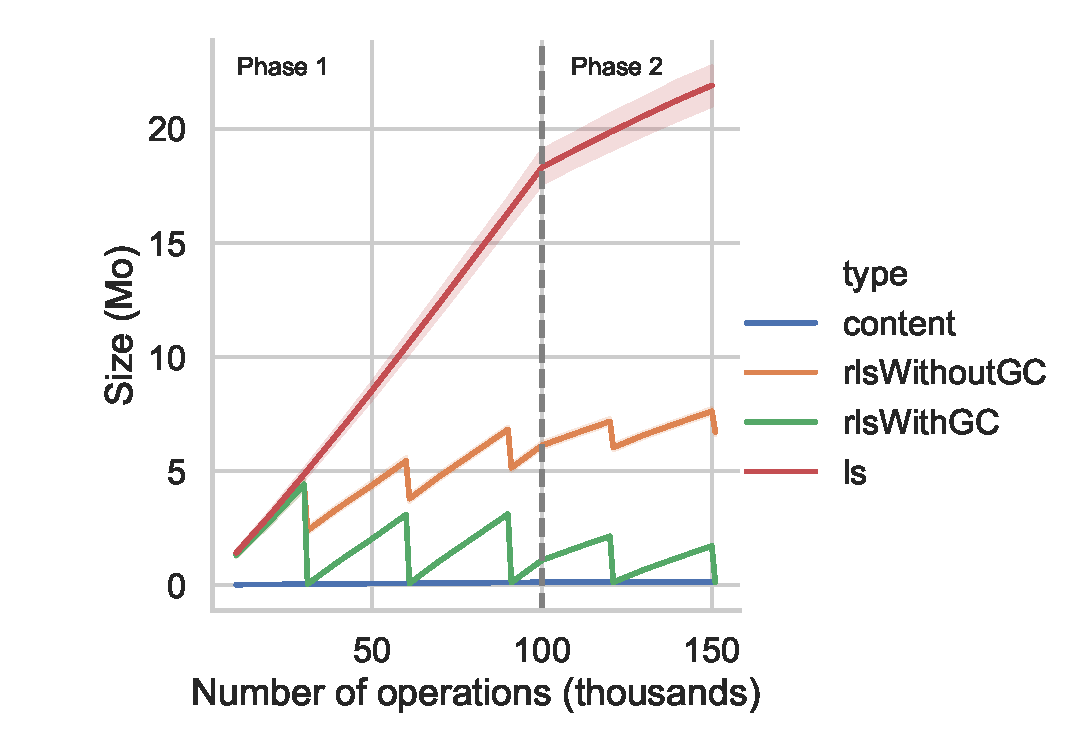
\includegraphics[width=\columnwidth]{img/snapshots-sizes.pdf}
    \caption{Evolution of the size of the document}
    \label{fig:evolution-document-size}
\end{figure}

\begin{sloppypar}
The dotted green line illustrates the growth of the RenamableLogootSplit document in its best-case scenario where \emph{rename} operations become stable as soon as they are issued.
Former states can then be garbage collected safely, maximising the benefits of the \emph{renaming} mechanism.
In this case, we observe that \emph{rename} operations reset the overhead of the data structure and eventually reduce by hundred times the document size compared to LogootSplit.
\end{sloppypar}

The dashed orange line represents RenamableLogootSplit worst-case scenario.
Here, we assume that \emph{rename} operations never become causally stable and that nodes have to store former states forever.
However, obtained results show that RenamableLogootSplit still outperforms LogootSplit and reduces by 66\% the overhead.
This outcome is due to the change of data structure used to represent the state that takes place when applying a \emph{rename} operation.
To perform updates efficiently, our implementation uses an AVL, a self-balancing tree, to represent the sequence.
However, we no longer update the former state once it has been renamed but only query it to transform concurrent operations.
We thus store it as an array, a more efficient memory-wise data structure, to save space.

\paragraph{Integration times of standard operations}

We also measure the impact of the renaming mechanism on the integration times of \emph{insert} and \emph{remove} operations.

\autoref{fig:evolution-integration-time-local-insert-remove} displays the integration times of local operations while \autoref{fig:evolution-integration-time-remote-insert-remove} exhibits remote ones.
In both cases, the light orange boxplots correspond to integration times of LogootSplit while dark blue ones to the integration times of RenamableLogootSplit.
The results show that the \emph{renaming} mechanism allows to reduce the integration times of future operations.

\begin{figure}[ht!]
    \begin{subfigure}{\columnwidth}
        \centering
        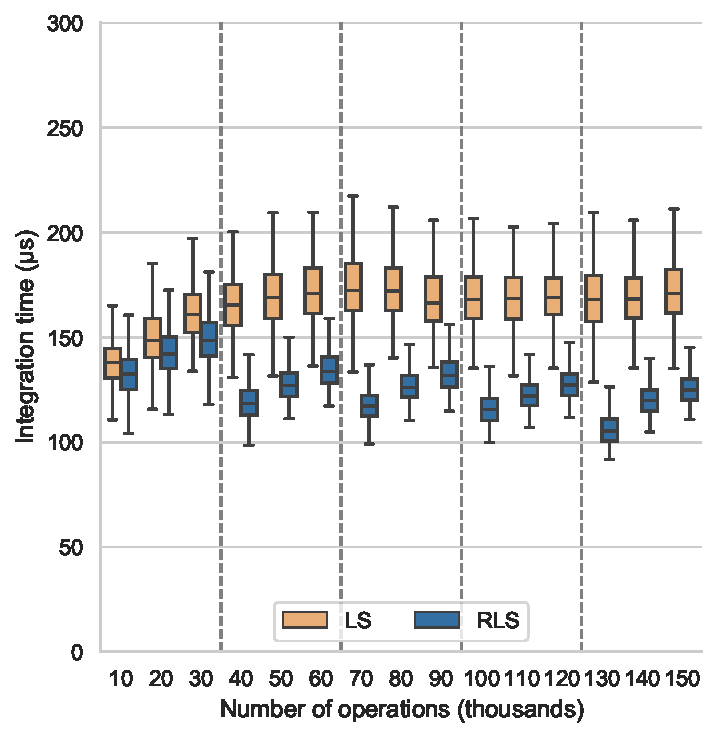
\includegraphics[width=0.9\columnwidth]{img/integration-time-boxplot-local-operations-without-outliers.pdf}
        \caption{Local operations}
        \label{fig:evolution-integration-time-local-insert-remove}
    \end{subfigure}
    \begin{subfigure}{\columnwidth}
        \centering
        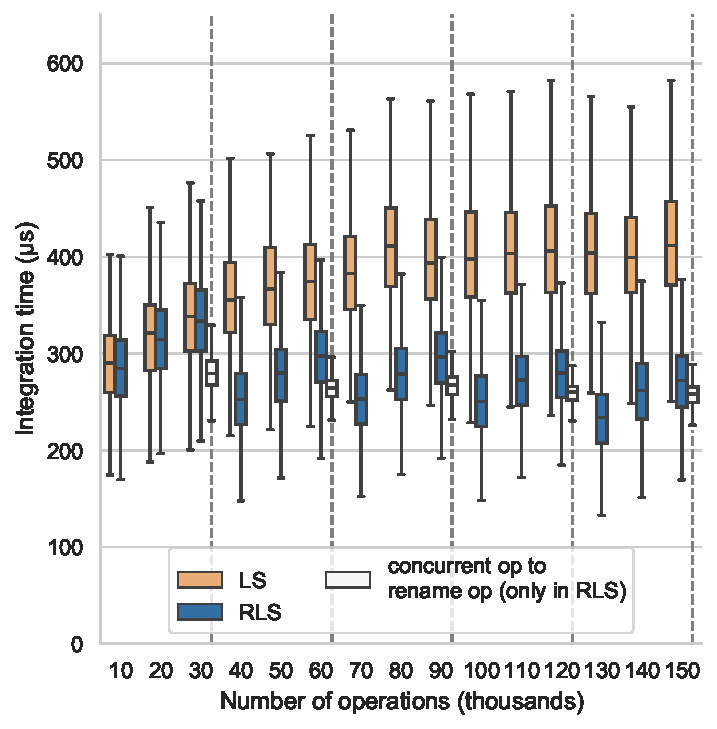
\includegraphics[width=0.9\columnwidth]{img/integration-time-boxplot-remote-operations-without-outliers.pdf}
        \caption{Remote operations}
        \label{fig:evolution-integration-time-remote-insert-remove}
    \end{subfigure}
    \caption{Integration time of standard operations}
    \label{fig:evolution-integration-time-insert-remove}
\end{figure}

In \autoref{fig:evolution-integration-time-remote-insert-remove}, the white boxplots display the integration times of concurrent operations to a \emph{rename} one.
As illustrated in \autoref{sec:dealing-with-concurrent-updates}, these operations require to be transformed before being applied to the renamed state.
The results presented here show that the whole process is actually faster than applying them directly on the former state.

\paragraph{Integration time of \emph{rename} operation}

Finally, we measure the integration times of \emph{rename} operations according to the size of the document.
Results are displayed in \autoref{fig:evolution-integration-time-rename} where the blue line corresponds to the integration times of local \emph{rename} operations while the dashed orange one corresponds to the integration times of remote ones.

\begin{figure}[ht!]
    \centering
    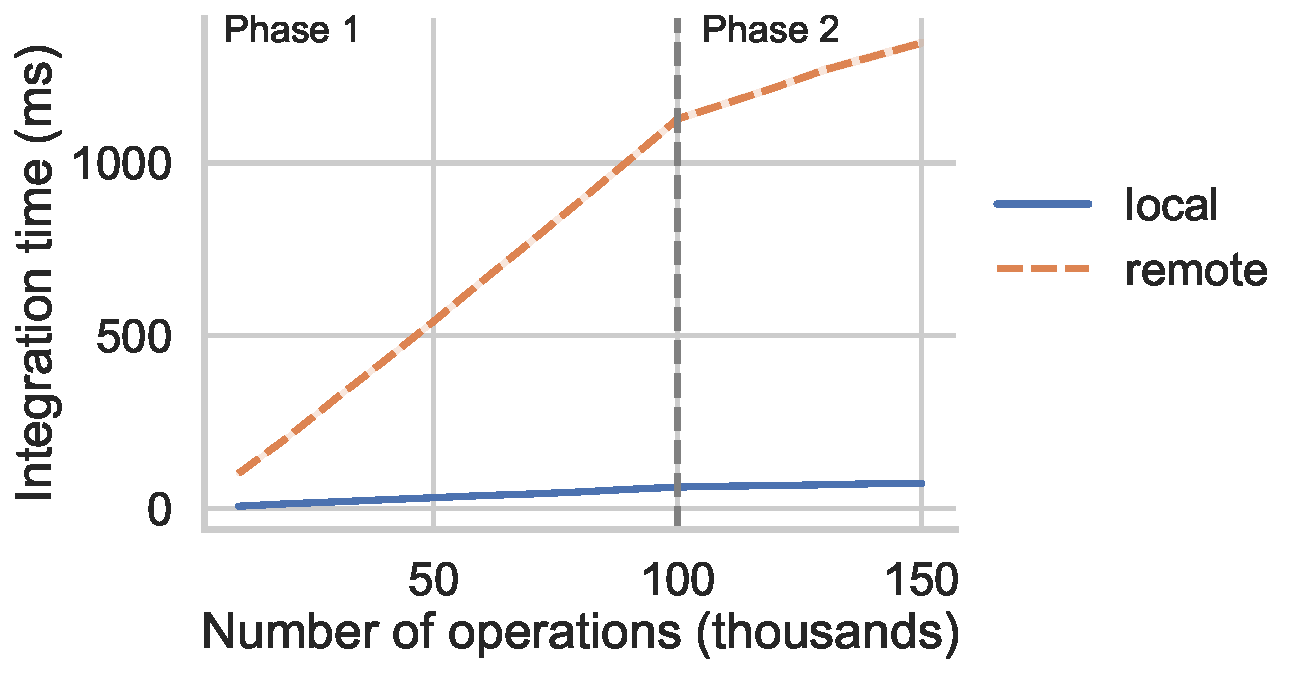
\includegraphics[width=0.9\columnwidth]{img/integration-time-rename.pdf}
    \caption{Integration time of rename operations}
    \label{fig:evolution-integration-time-rename}
\end{figure}

The main result of this benchmark is that the unit of time used when applying \emph{rename} operations is in hundreds of milliseconds.
It is necessary to take this into account when designing the strategy used to trigger \emph{rename} operations in order to minimise the impact of integration times on the user experience.

% In this section, we presented our experimental results.
% These results demonstrate that RenamableLogootSplit outperforms LogootSplit and can reduce by hundreds the size of the document.
% They also show that
% However, it comes at the price of an expensive but infrequent \emph{rename} operation.
% In the next section, we present related work and compare our approach to them.

\section{Related work}

\label{sec:related-work}

Several approaches have been proposed to reduce the growth of variable-size identifiers.
However, to the best of our knowledge, no work has been presented to decrease the number of blocks generated.

\subsection{The core-nebula approach}

In \cite{letia:hal-01248270,zawirski:hal-01248197}, authors design for Treedoc \cite{5158449} a renaming mechanism to reassign shorter identifiers to elements.
Nodes rely on a consensus mechanism to trigger the renaming and a catch-up protocol to handle concurrent updates.
Since consensus algorithms are costly in large-scale distributed systems with churn, \citet{letia:hal-01248270} introduce a two-tier architecture.
Nodes are splitted between the \emph{core}, a set of stable and highly connected nodes, and the \emph{nebula} made of the remaining ones.
Only members of the \emph{core} participate in the consensus leading to the renaming.

While quite similar, our approach differs on several aspects.
First, in the \emph{core-nebula} approach, nodes from the \emph{core} are unable to integrate concurrent operations to the \emph{rename} one.
Nodes from the \emph{nebula} have to use the catch-up protocol to transform their concurrent operations and to re-broadcast them.
It requires additional communications and introduces some delay in the collaboration.
In our approach, every node is able to transform and to integrate operations from past epochs directly.

Second, we designed RenamableLogootSplit with fully distributed systems in mind.
Nodes can issue \emph{rename} operations without coordination and use \emph{operational transformation} to resolve conflicts.
However, to simplify the system, it is possible to adopt the \emph{core-nebula} approach to prevent nodes from issuing concurrent \emph{rename} operations.

\subsection{The LSEQ approach}

In \cite{nedelec_2013_lseq,doi:10.1002/cpe.4108}, \citeauthor{nedelec_2013_lseq} introduce another approach to address the identifiers growth issue: LSEQ.
Its insight consists in combining several strategies to generate new identifiers.
It enables LSEQ to reduce the growth of identifiers from a linear progression to a polylogarithmic one.

However, LSEQ does not prevent each inserted element to introduce its own overhead.
The document continues to inflate with each insertion.
On the other hand, our approach allows the metadata of the data structure to be periodically reset, regardless of the number of elements.

As with the \emph{core-nebula} approach, it is possible to combine the LSEQ approach with ours.
The identifier allocation strategies of LSEQ would allow to reduce the growth of identifiers between \emph{rename} operations.
It would enable to reduce the frequency of the expensive \emph{rename} operation without deteriorating the performance of the data structure.

\section{Conclusions and future work}
\label{sec:conclusion}

\begin{sloppypar}
In this paper, we introduced a novel Sequence \ac{CRDT} belonging to the variable-size identifiers approach: RenamableLogootSplit.
This new data structure embeds a renaming mechanism in its specification.
It enables nodes to reassign shorter identifiers to elements and group them into one block to minimise the metadata.
Experiments results provided an empirical validation of the correctness of RenamableLogootSplit and showed that it reduces the overhead of the data structure in both best-case (by hundreds times) and worst-case scenarios.
\end{sloppypar}

Regarding future work, we would like to present a formal proof of the correctness of RenamableLogootSplit.
Another research trail would be to investigate how OT techniques can be integrated within \acp{CRDT} to design more complex data types.

% A working trail/research trail
% Comment les techniques d'OT s'insèrent dans les CRDTs

Additionally, we now have to design an efficient strategy used to trigger \emph{rename} operations while minimising their impact on the user experience.
User behaviour studies, inspired by \cite{ignat:hal-01088815,ignat:hal-01238831}, could be led in the context of real-time collaborative writing to set an acceptable upper-bound to their integration times.

Finally, we designed RenamableLogootSplit with fully distributed systems in mind.
However, for the sake of brevity, we presented it in this paper under the assumption that no concurrent \emph{rename} operations were issued.
This scenario is actually akin to systems in which nodes synchronise to trigger the renaming mechanism.
In a future work, we will introduce and evaluate the additional steps required to use RenamableLogootSplit in its original settings.

\bibliography{ref}

\end{document}
